\documentclass[../Main.tex]{subfiles}
\begin{document}
Chapter 3 will provide a thorough examination of the system characteristics and architecture of our novel social login system. This chapter provides a fundamental understanding of the complex mechanisms and distinguishing characteristics that set our system apart in the decentralized oracle network field. Next, the chapter will provide a detailed description of the system architecture. The social login system has been divided into three sub-processes to enhance clarity and address its inherent complexity. This section will provide a comprehensive explanation of each sub-process, emphasizing its distinct functionalities and responsibilities within the overall system flow. By breaking down the system into separate phases, readers can understand the specific steps required to process a user's request and smoothly execute the social login mechanism.
\section{System's characteristics}
This study examines the efficacy and adaptability of a system that utilizes conventional social login methods to augment the UX of DApps. The following characteristics can be more detailed: \\
\indent\textbf{Security} - combining the potential benefits of blockchain smart-contract, SSS, and Pedersen DKG protocol. The security infrastructure of the system is established upon the utilization of blockchain smart contracts. Programmable contracts, operating on a decentralized network, guarantee the attributes of transparency, immutability, and tamper-proof execution of operations. Shamir secret sharing is used to fortify the protection of cryptographic keys and other forms of private information. This method entails breaking up a secret into smaller pieces and giving them to several parties. The Petersen DKG protocol distributes and secures cryptographic key generation, ensuring system security. This system lets a group of people generate a shared cryptographic key without anyone having the full key. 

\indent\textbf{Efficacy and adaptability} - By leveraging blockchain's decentralized nature, Web3Auth eliminates the reliance on centralized identity providers, reducing the potential for single points of failure and enhancing security. Additionally, blockchain-based identity systems enable instant verification of user credentials, eliminating the need for lengthy verification processes and reducing transaction times. The open solution's architecture enables seamless integration with any DApps, making it easier for developers to adopt and implement with their products. 

\indent\textbf{User-friendly} - This solution supports popular authentication mechanisms such as social login which are widely used in the traditional web. This familiarity allows users to leverage their existing accounts and authentication methods, reducing the learning curve and providing a seamless transition into the Web3 space. Users can easily authenticate their identities across multiple DApps using a unified and standardized protocol, without the need to remember and manage multiple usernames and passwords. This eliminates the hassle of creating and maintaining numerous accounts, making the user experience more streamlined and efficient.

\indent\textbf{Scalability} - Compatible with any type of social authentication, including Facebook, Google, and Twitter. Utilizing a decentralized architecture increased the request's performance and volume by spreading it across multiple executors and parallel handling processes.
\newpage
\section{Overall of system}
\begin{figure}[H]
 \centering
 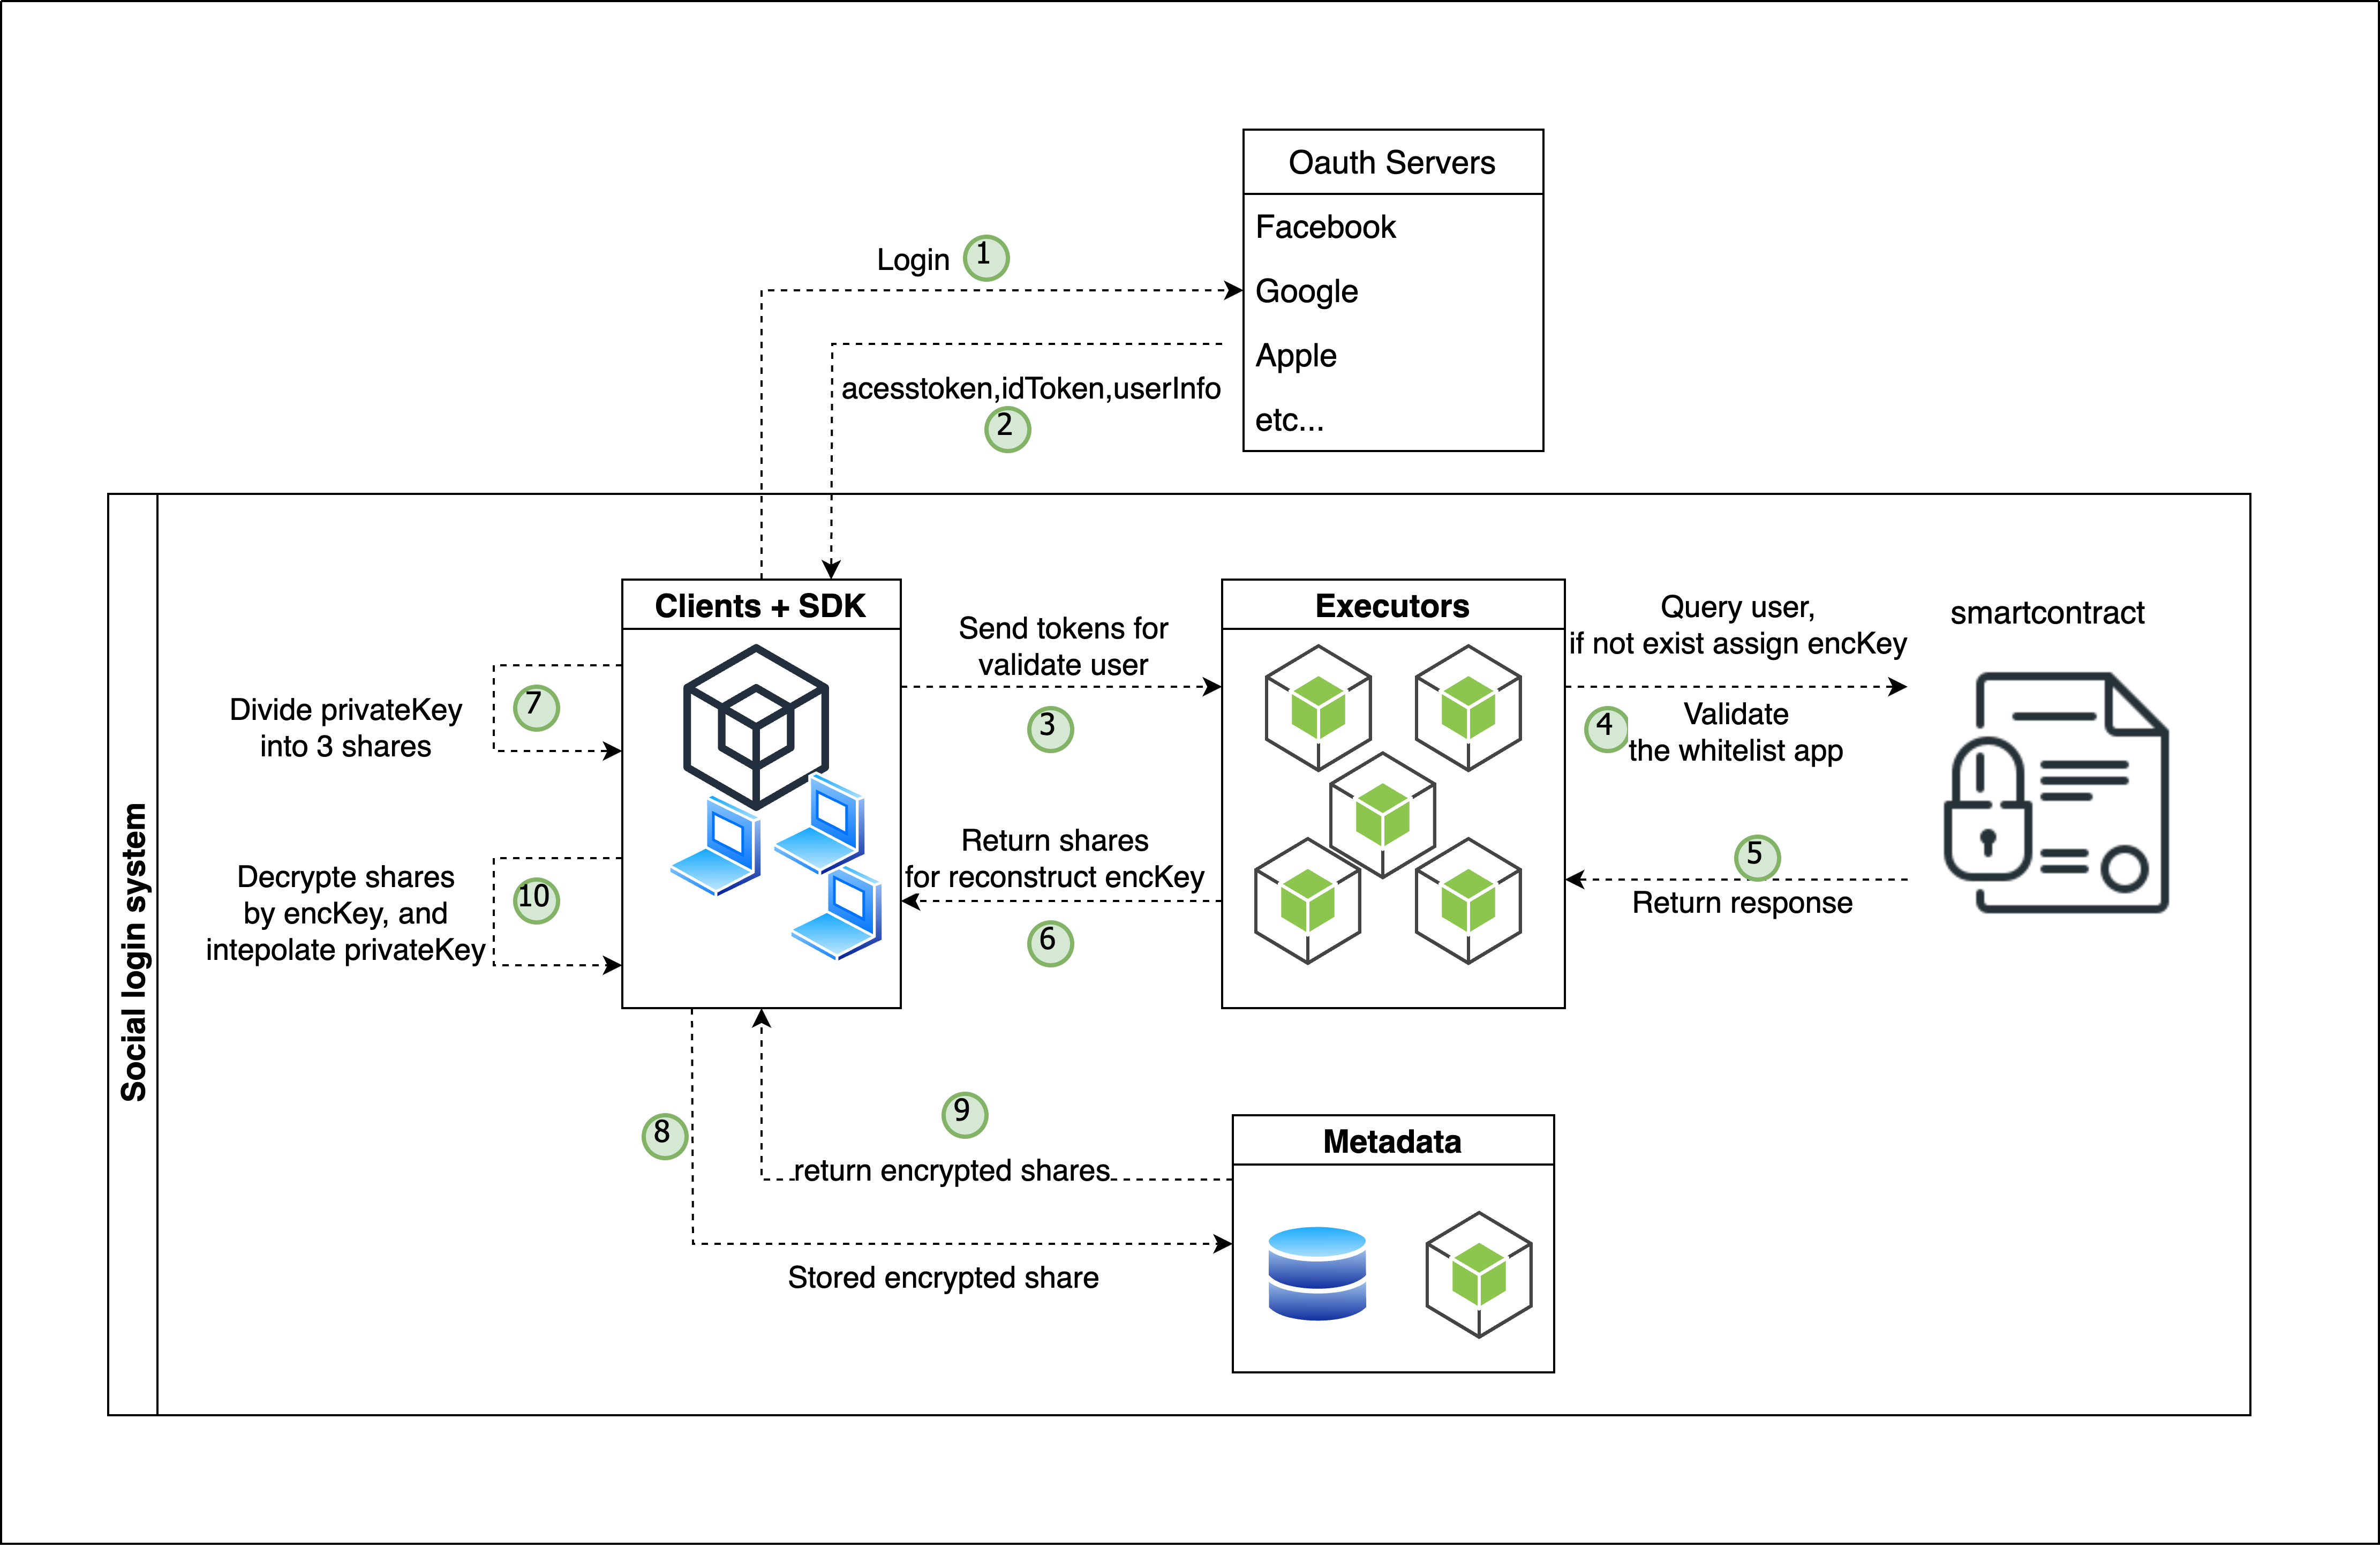
\includegraphics[scale=0.1]{Figure/OverallSocialLoginSystem.png}
    \caption{Overall the system}
    \label{fig:OverallSystem}
\end{figure}
Figure \ref{fig:OverallSystem} illustrates the comprehensive flow of a user's request when interacting with the social login system. Due to the intricacy of this process, it has been broken down into three distinct sub-processes, each serving a particular purpose. This division aims to enhance clarity and provide a more in-depth understanding of the overall system's functionality and interactions.
The user's journey commences with the initiation of a request, where they opt to utilize the social login feature. Subsequently, the first sub-process comes into play, responsible for validating the user's input and ensuring the security of the request. Once the request passes through this validation phase, it proceeds to the second sub-process, where the social login credentials are authenticated against the relevant provider's authentication system.
Upon successful authentication, the third sub-process takes charge, executing the logic of constructing the encryption key and the assignment key. With these keys securely generated, the system progresses further, utilizing smart contracts and blockchain technology to store and safeguard the user's data throughout the duration of the chain's active state.

\subsection{Auth0 connection}
\begin{figure}[H]
 \centering
 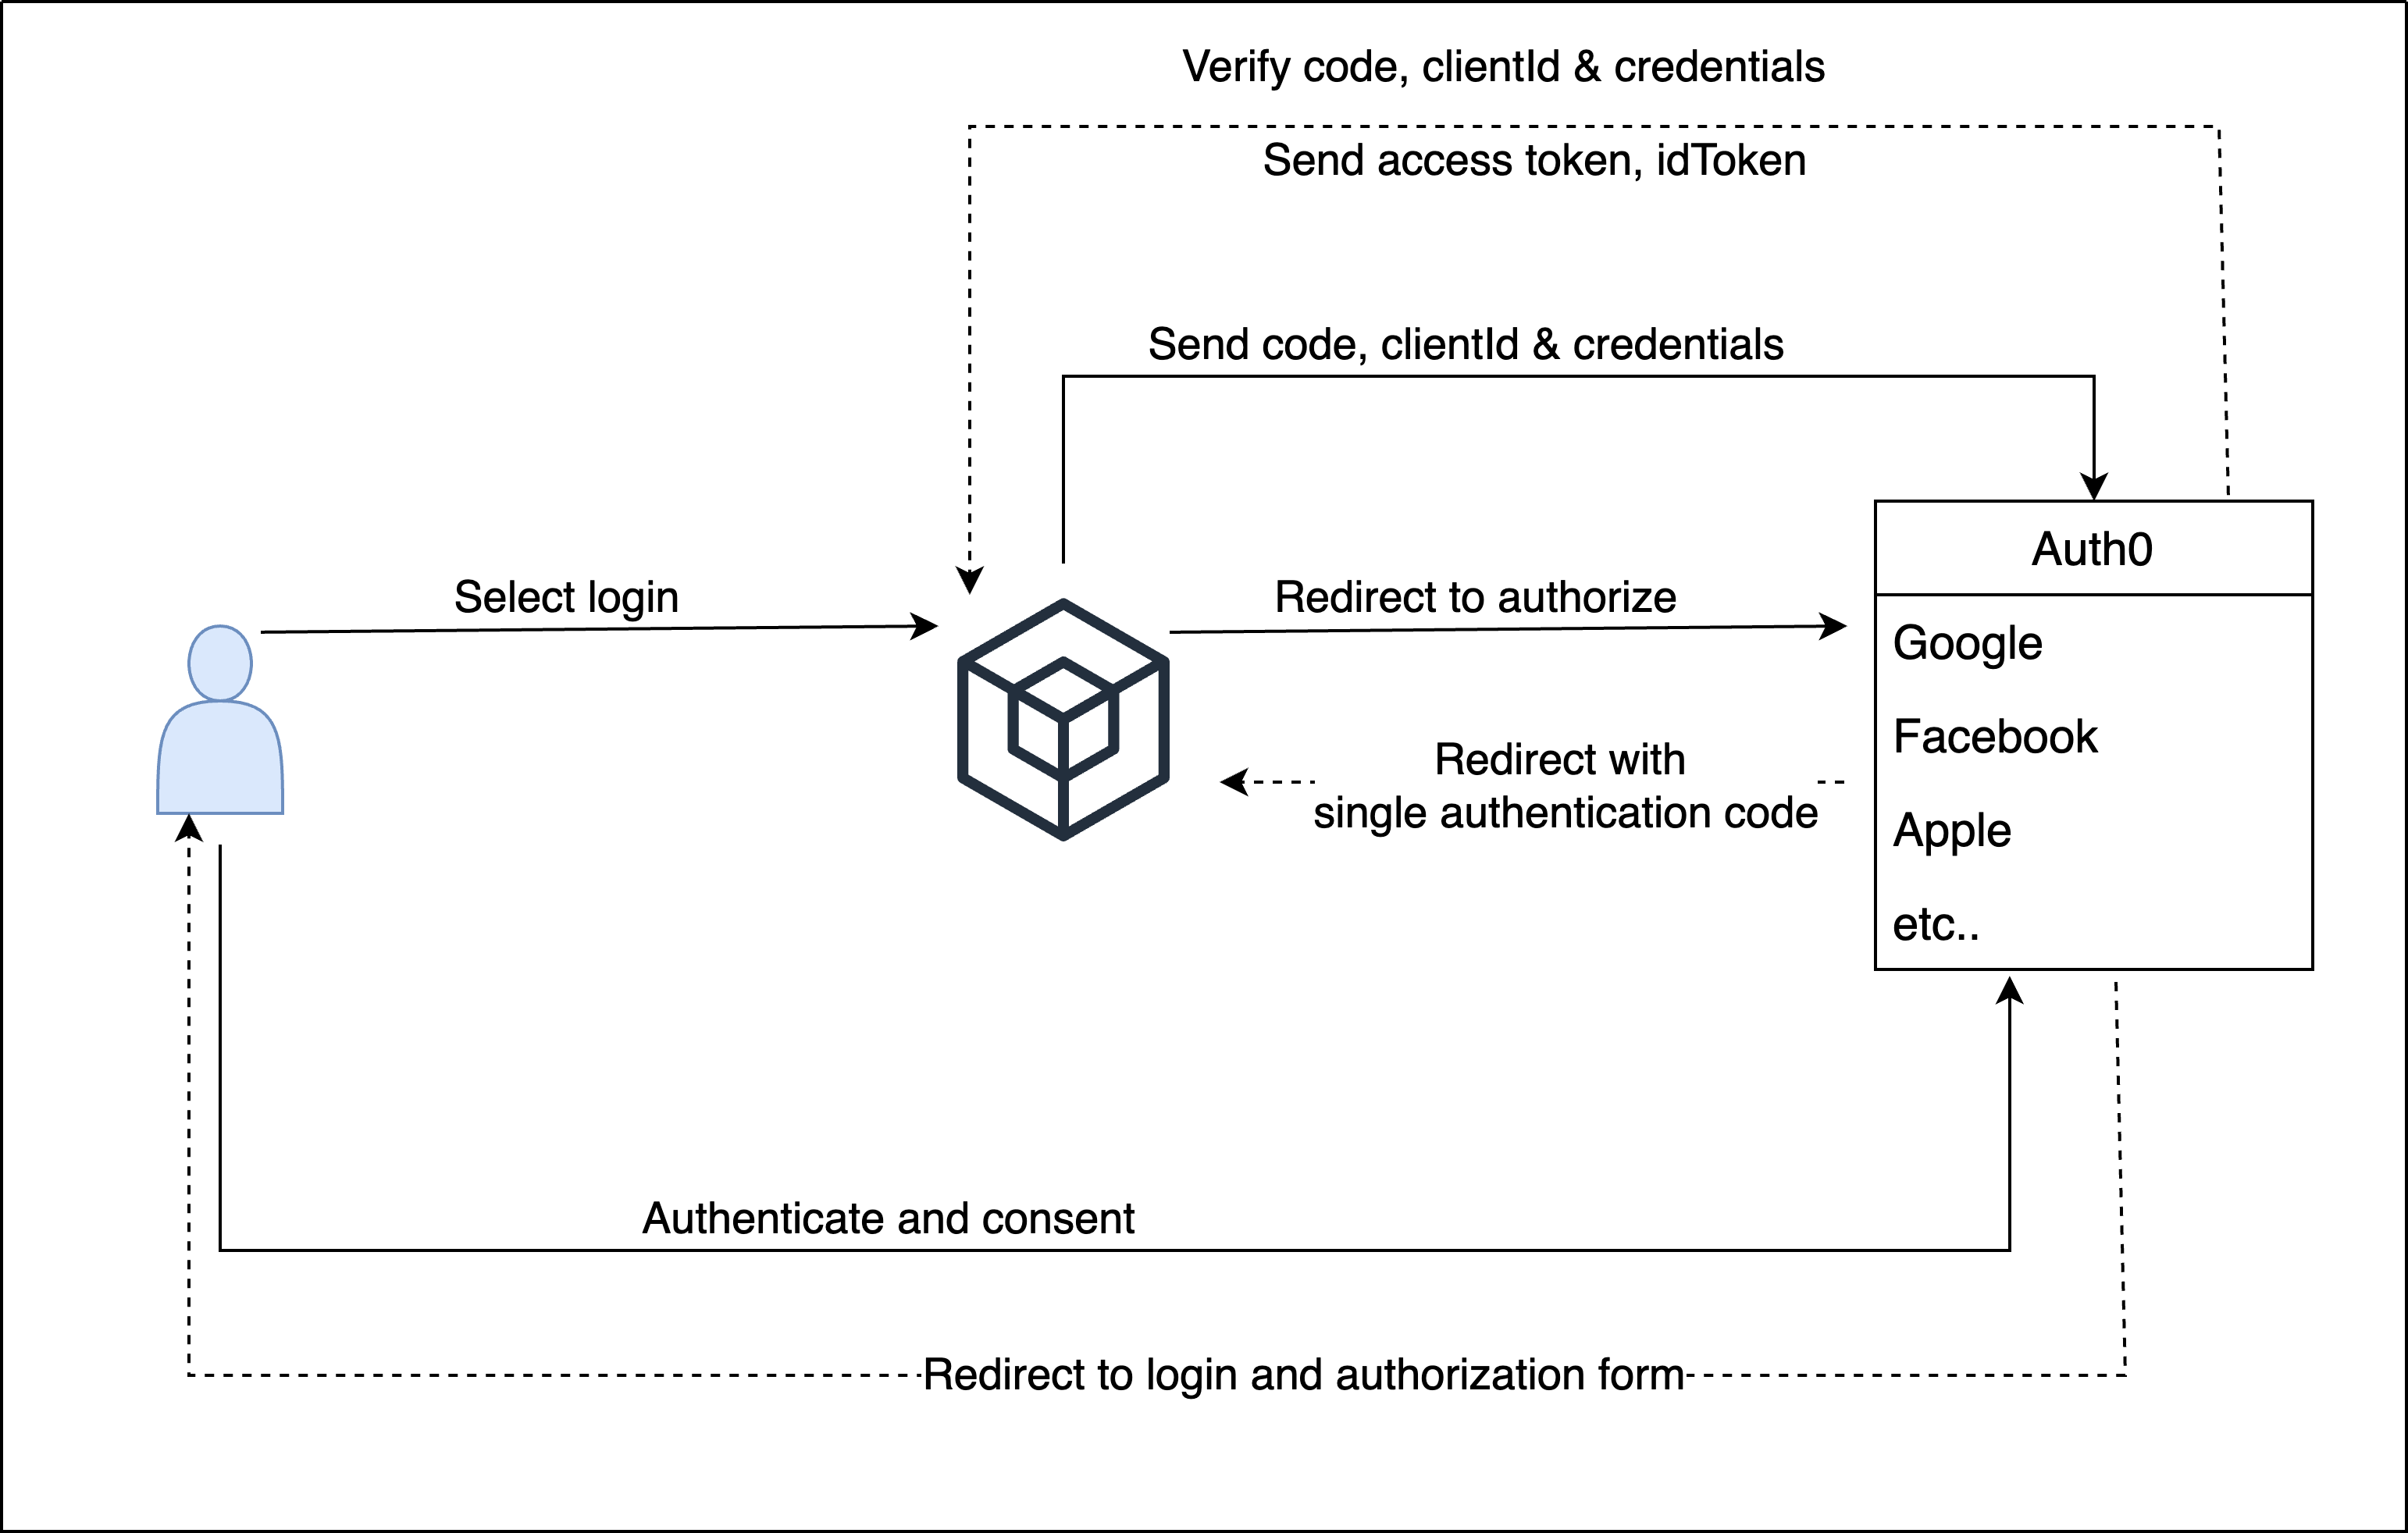
\includegraphics[scale=0.14]{Figure/Oauth-connection.png}
    \caption{Auth0 connection}
    \label{fig:Auth0-connection}
\end{figure}
Figure \ref{fig:Auth0-connection} is a graphical representation of the Auth0 authentication and authorization solution. When the user selects the intended authentication type within the application, the process begins. This could be accomplished using a traditional username and password or other methods, such as social registration with Google or Facebook. After selecting the authentication type, the application redirects the user to the Auth0 server's authorization endpoint. The user is then presented with a login and authorization prompt, where they can securely authenticate themselves and grant any necessary permissions. This step ensures that only authorized users have access to the application's resources and can conduct particular actions. The Auth0 server redirects the user back to the application along with an authorization code following successful authentication and assent. The application then exchanges this authorization code, along with its own credentials and client ID, with the Auth0 server's token endpoint. The Auth0 server verifies the supplied information, including the authorization code, credentials, and client ID, with extreme precision. If the verification procedure is effective, the server issues both an access token and an ID token to the application. Different purposes are served by these identifiers during the authentication and authorization process. The application uses the access token to authenticate subsequent inquiries on the user's behalf. It serves as evidence of authorization and grants access to protected resources or API endpoints. This token is typically included in API request parameters, allowing for secure and seamless communication between the application and server. The ID token, on the other hand, contains vital user information that can be used for identification and authentication. It may contain information such as the user's email address, identity, and other pertinent characteristics. The ID token enables the application to recognize the user and tailor the user's experience within the application. Auth0's extensive features make it a robust and dependable authentication and authorization solution. By leveraging secure protocols and industry best practices, Auth0 assures the privacy and integrity of user data through a secure and efficient process.
\subsection{Requesting encKey for Executors}
\begin{figure}[H]
 \centering
 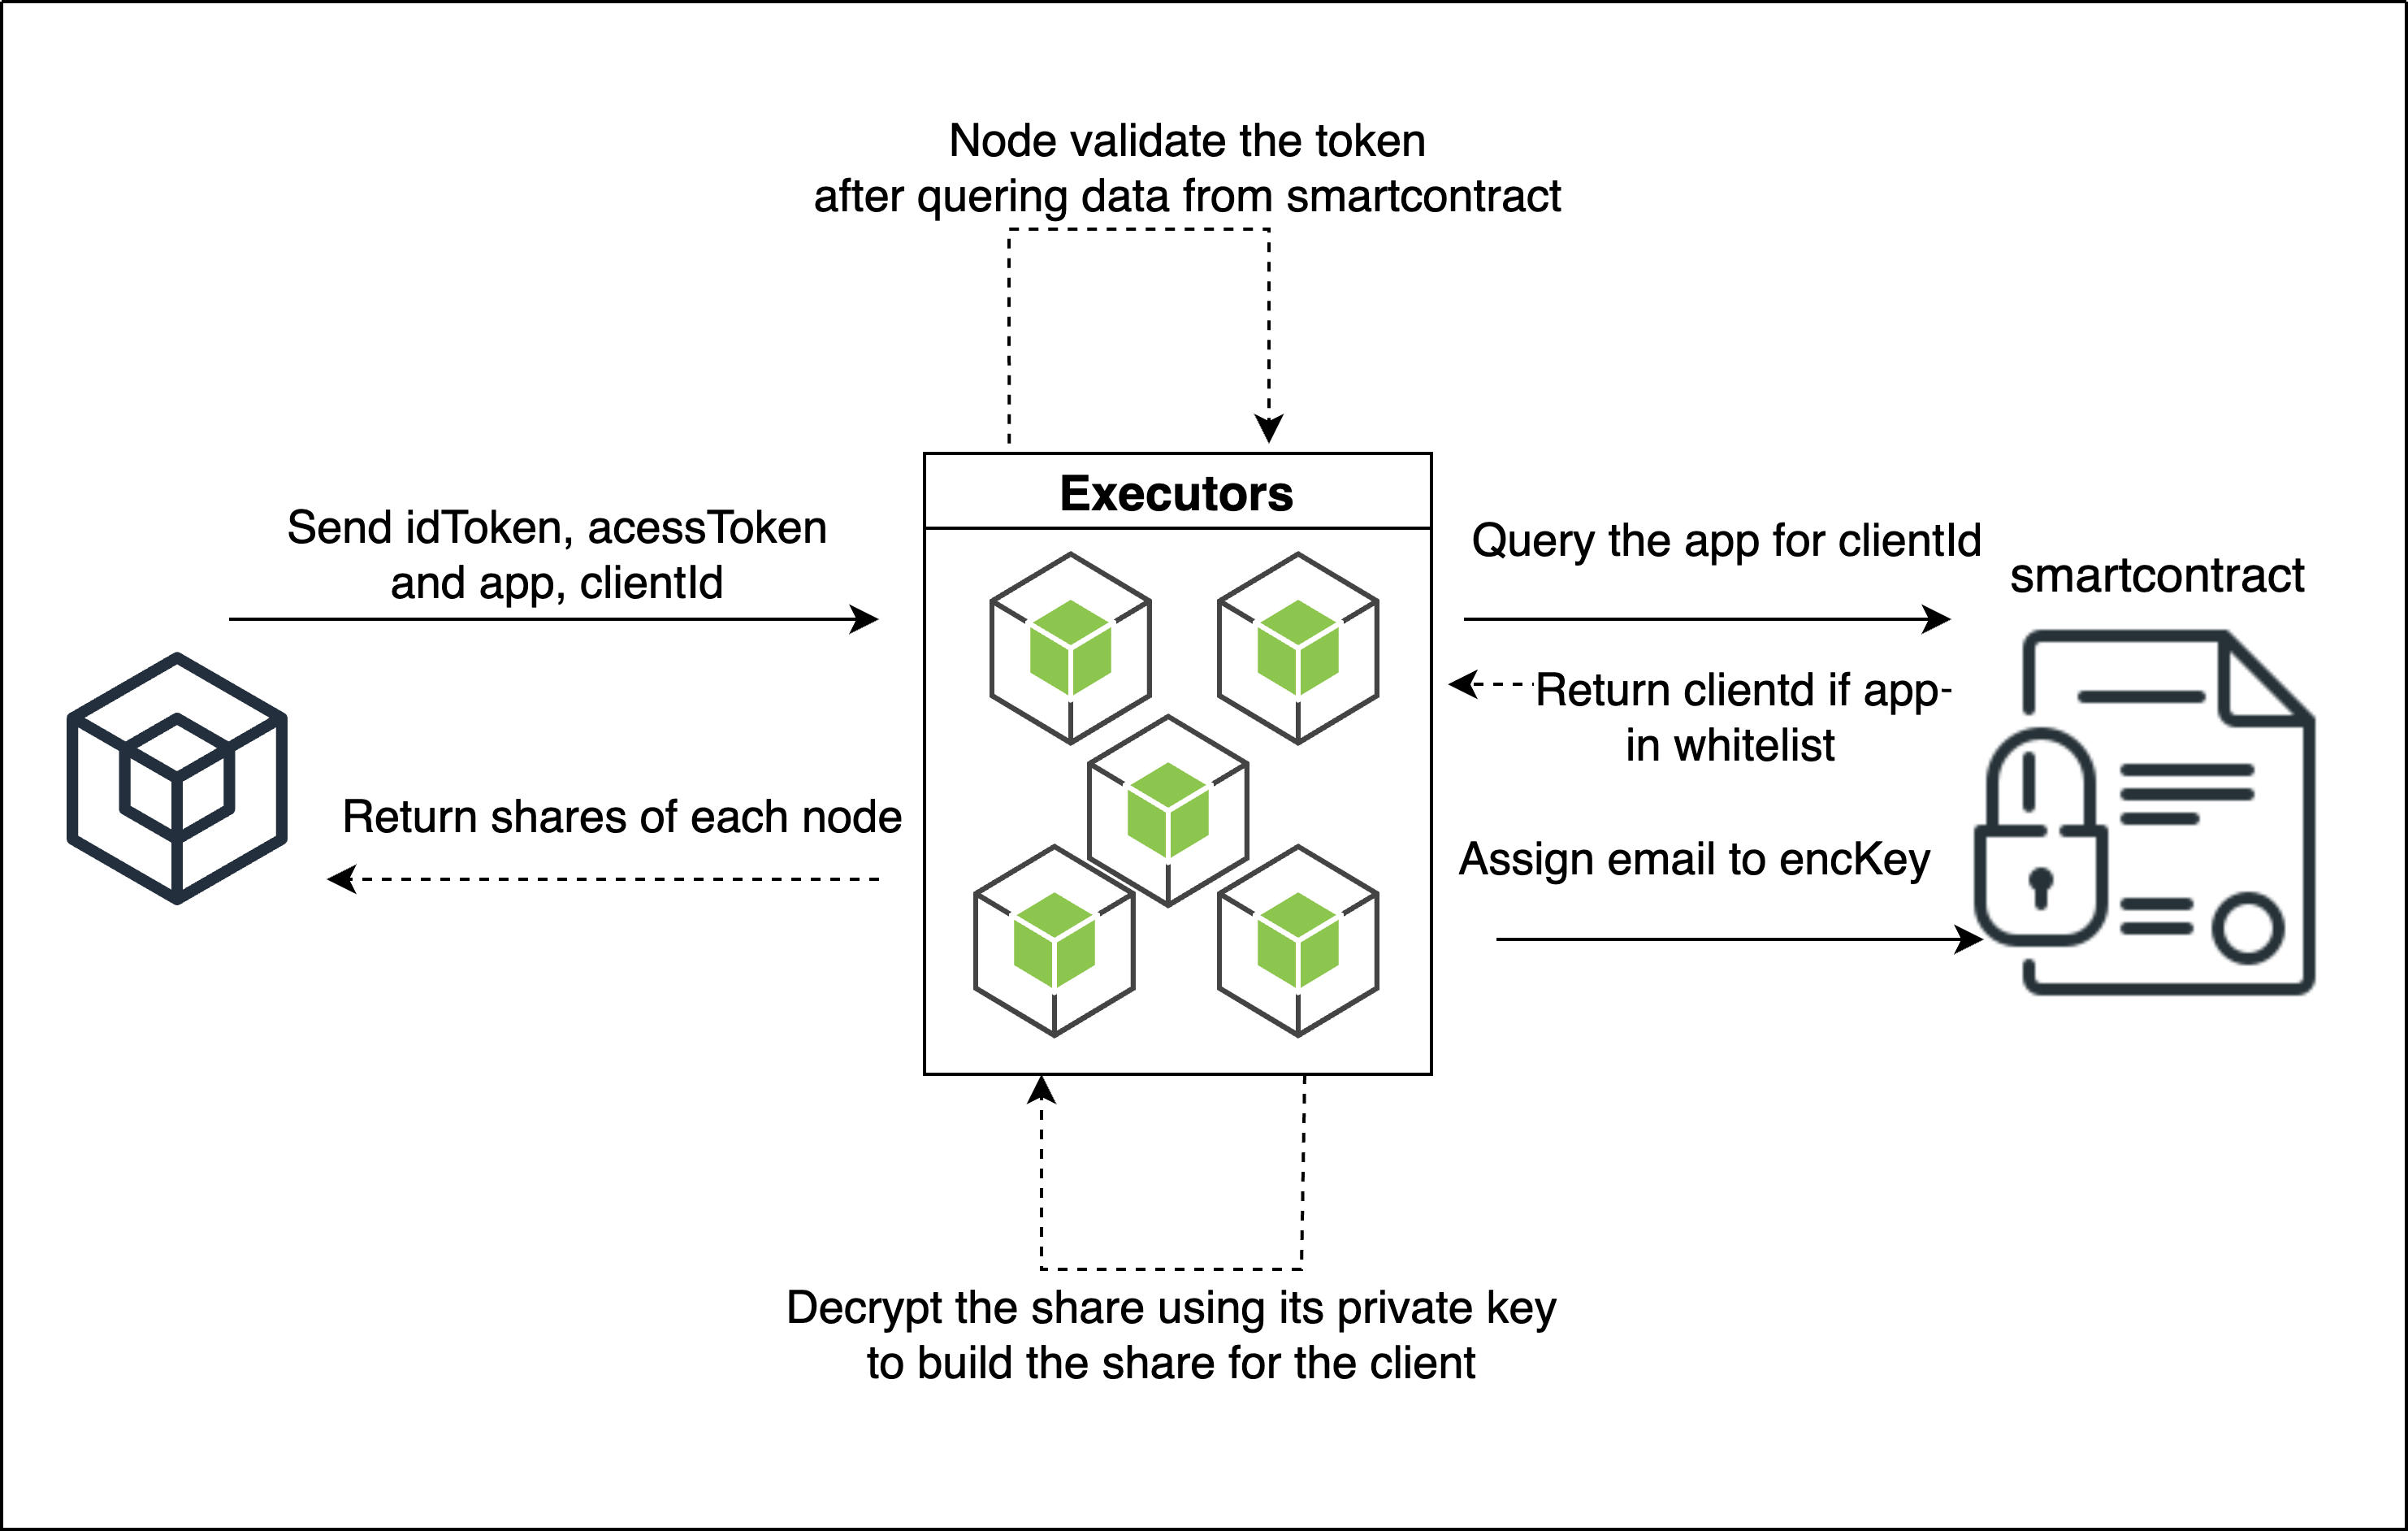
\includegraphics[scale=0.14]{Figure/request-share.png}
    \caption{Request assign the share}
    \label{fig:request-share}
\end{figure}
Multiple stages, described in Figure \ref{fig:request-share}, are required to ensure secure and effective authentication and authorization. The SDK functions as the interface between the user's device and the system. The SDK sends the idToken or accessToken, as well as the appName and clientId, to the executors when the user initiates the authentication procedure. The executors play a vital role in authenticating the user's credentials and interacting with the smart contract in a secure manner. They begin by querying the smart contract to retrieve pertinent information regarding the accessed app. This information contains the essential authentication and authorization parameters and configuration data. The executors commence the validation procedure upon receiving the data from the smart contract. They validate the integrity and authenticity of the data extracted from the idToken or accessToken. This validation ensures that the user's credentials have not been altered during transmission and are legitimate. If the user attempting authentication is a new user, the executors generate a unique key for them. This key is securely associated with the user's authenticated email address and functions as a digital identifier. This phase ensures that each user within the system has a unique identifier. The executors then receive the shares encrypted by the smart contract in a secure manner. These shares are encrypted with the private keys of the nodes that participated in the distributed key generation procedure. The executors can decrypt the shares using their own private keys, ensuring that the process remains secure and confidential. After decrypting the shares, the executors reconstruct the final share and return it to the SDK. These shares are used as part of the authentication and authorization process, allowing the user to access and interact with decentralized applications (DApps) within the ecosystem in a secure manner. By adhering to this exhaustive and intricate procedure, the system ensures the authentication and authorization of users is efficient and secure. It leverages the capabilities of smart contracts, Shamir secret sharing, and the Petersen DKG protocol to provide a robust and dependable Web3 authentication solution.
\subsection{Generating and Storing Shares in Metadata}
\begin{figure}[H]
 \centering
 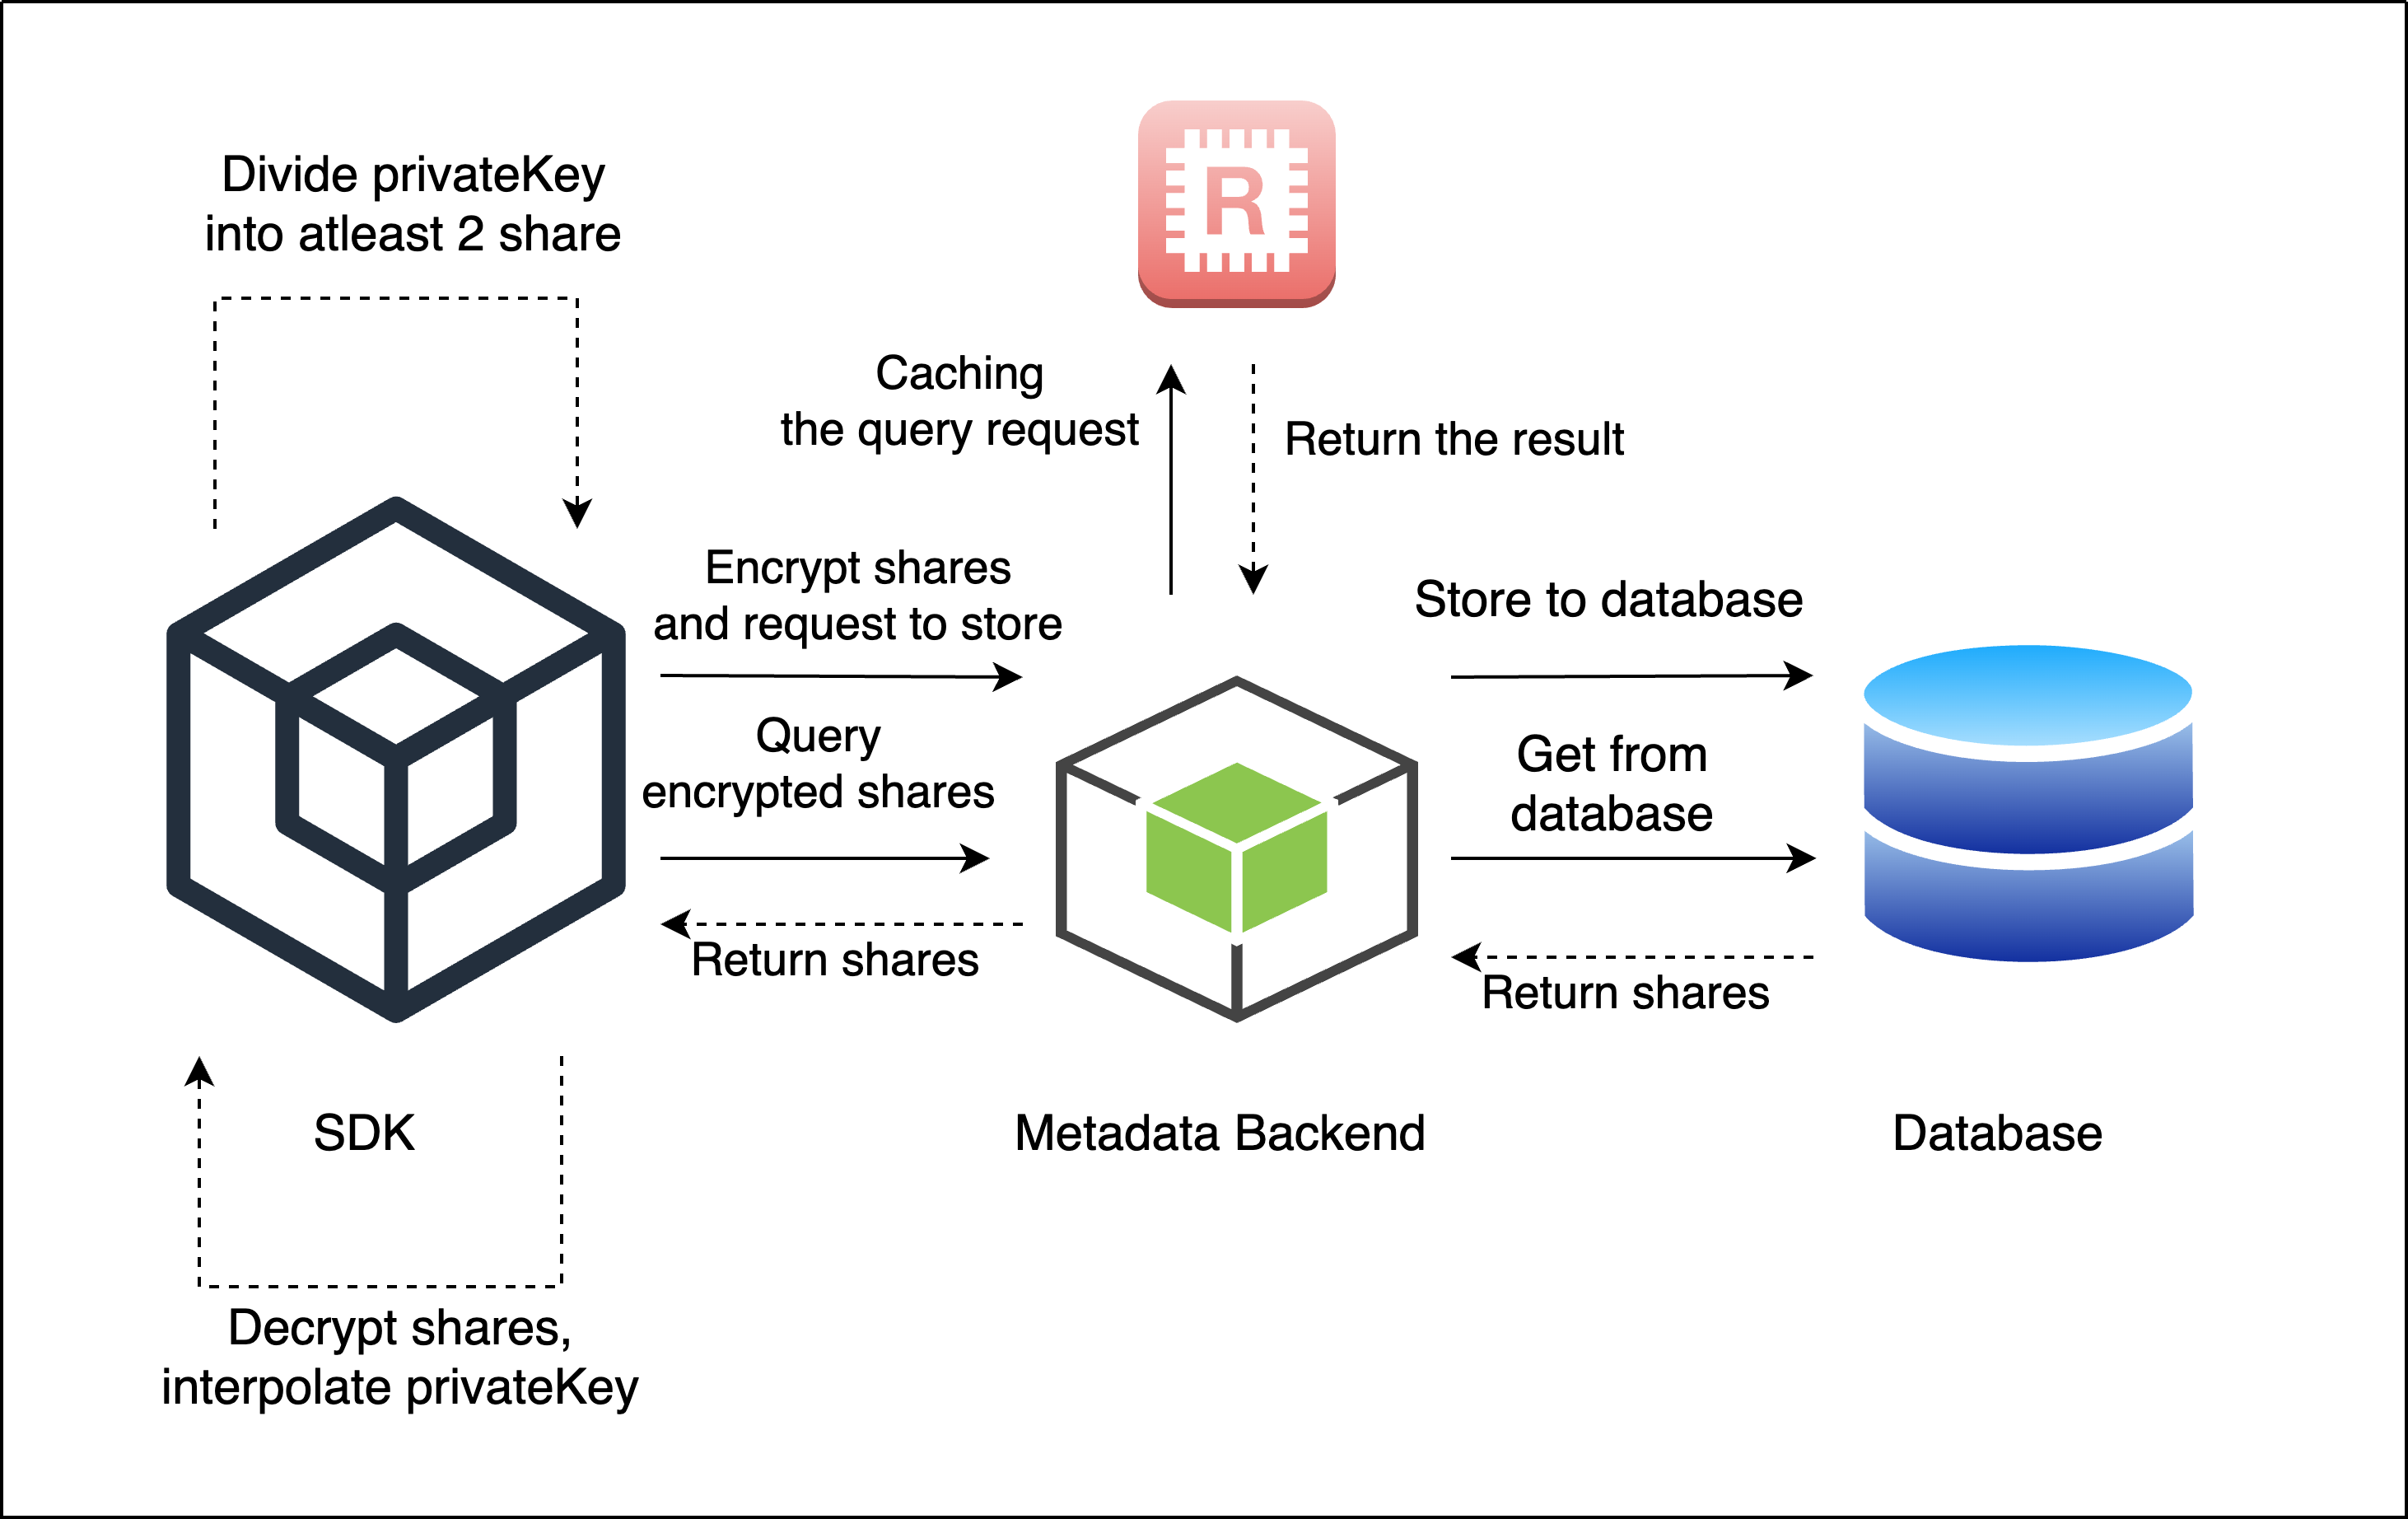
\includegraphics[scale=0.14]{Figure/generate-share.png}
 \caption{Generate & Reconstruct shares}
    \label{fig:generate-share}
\end{figure}
Reconstructing the private key in our system, as depicted in Figure \ref{fig:generate-share}, requires several phases to assure security and dependability. Beginning with Shamir's secret sharing scheme, the SDK divides the private key into at least two portions. Each share is encrypted to ensure its integrity and confidentiality. The encrypted shares are then transmitted to the metadata backend, where they are housed securely in the database. The SDK initiates a query request to the metadata repository when the need to reconstruct the private key arises. The backend retrieves from the database the encrypted shares associated with the specified user and application. The query result, including the encrypted shares, is cached in a Redis database to improve performance, enabling quicker retrieval for subsequent requests. After receiving the encrypted shares, the SDK initiates the reconstruction process. Each share is decrypted by the SDK using the corresponding decryption keys. These decryption keys are managed securely within the SDK, and only authorized processes have access to them. The SDK recovers the original confidential information contained within each share by decrypting the shares. The SDK combines the decrypted shares using interpolation algorithms, such as Lagrange interpolation, to generate the final private key. This method entails mathematical calculations that interpolate the missing portions of the private key using the available shares. The SDK effectively reconstructs the original private key through interpolation. Throughout this process, strong encryption algorithms and secure key management procedures guarantee the privacy and integrity of the private key. The use of Shamir's secret sharing scheme increases security by distributing the key across multiple shares, making it resistant to single points of failure or compromise. By implementing this comprehensive and secure reconstruction procedure, our system ensures the safe and dependable retrieval of the private key, allowing users to securely access their Web3 ecosystem accounts and conduct authorized actions.
\section{Asynchronous create encKey process}
\begin{figure}[H]
 \centering
 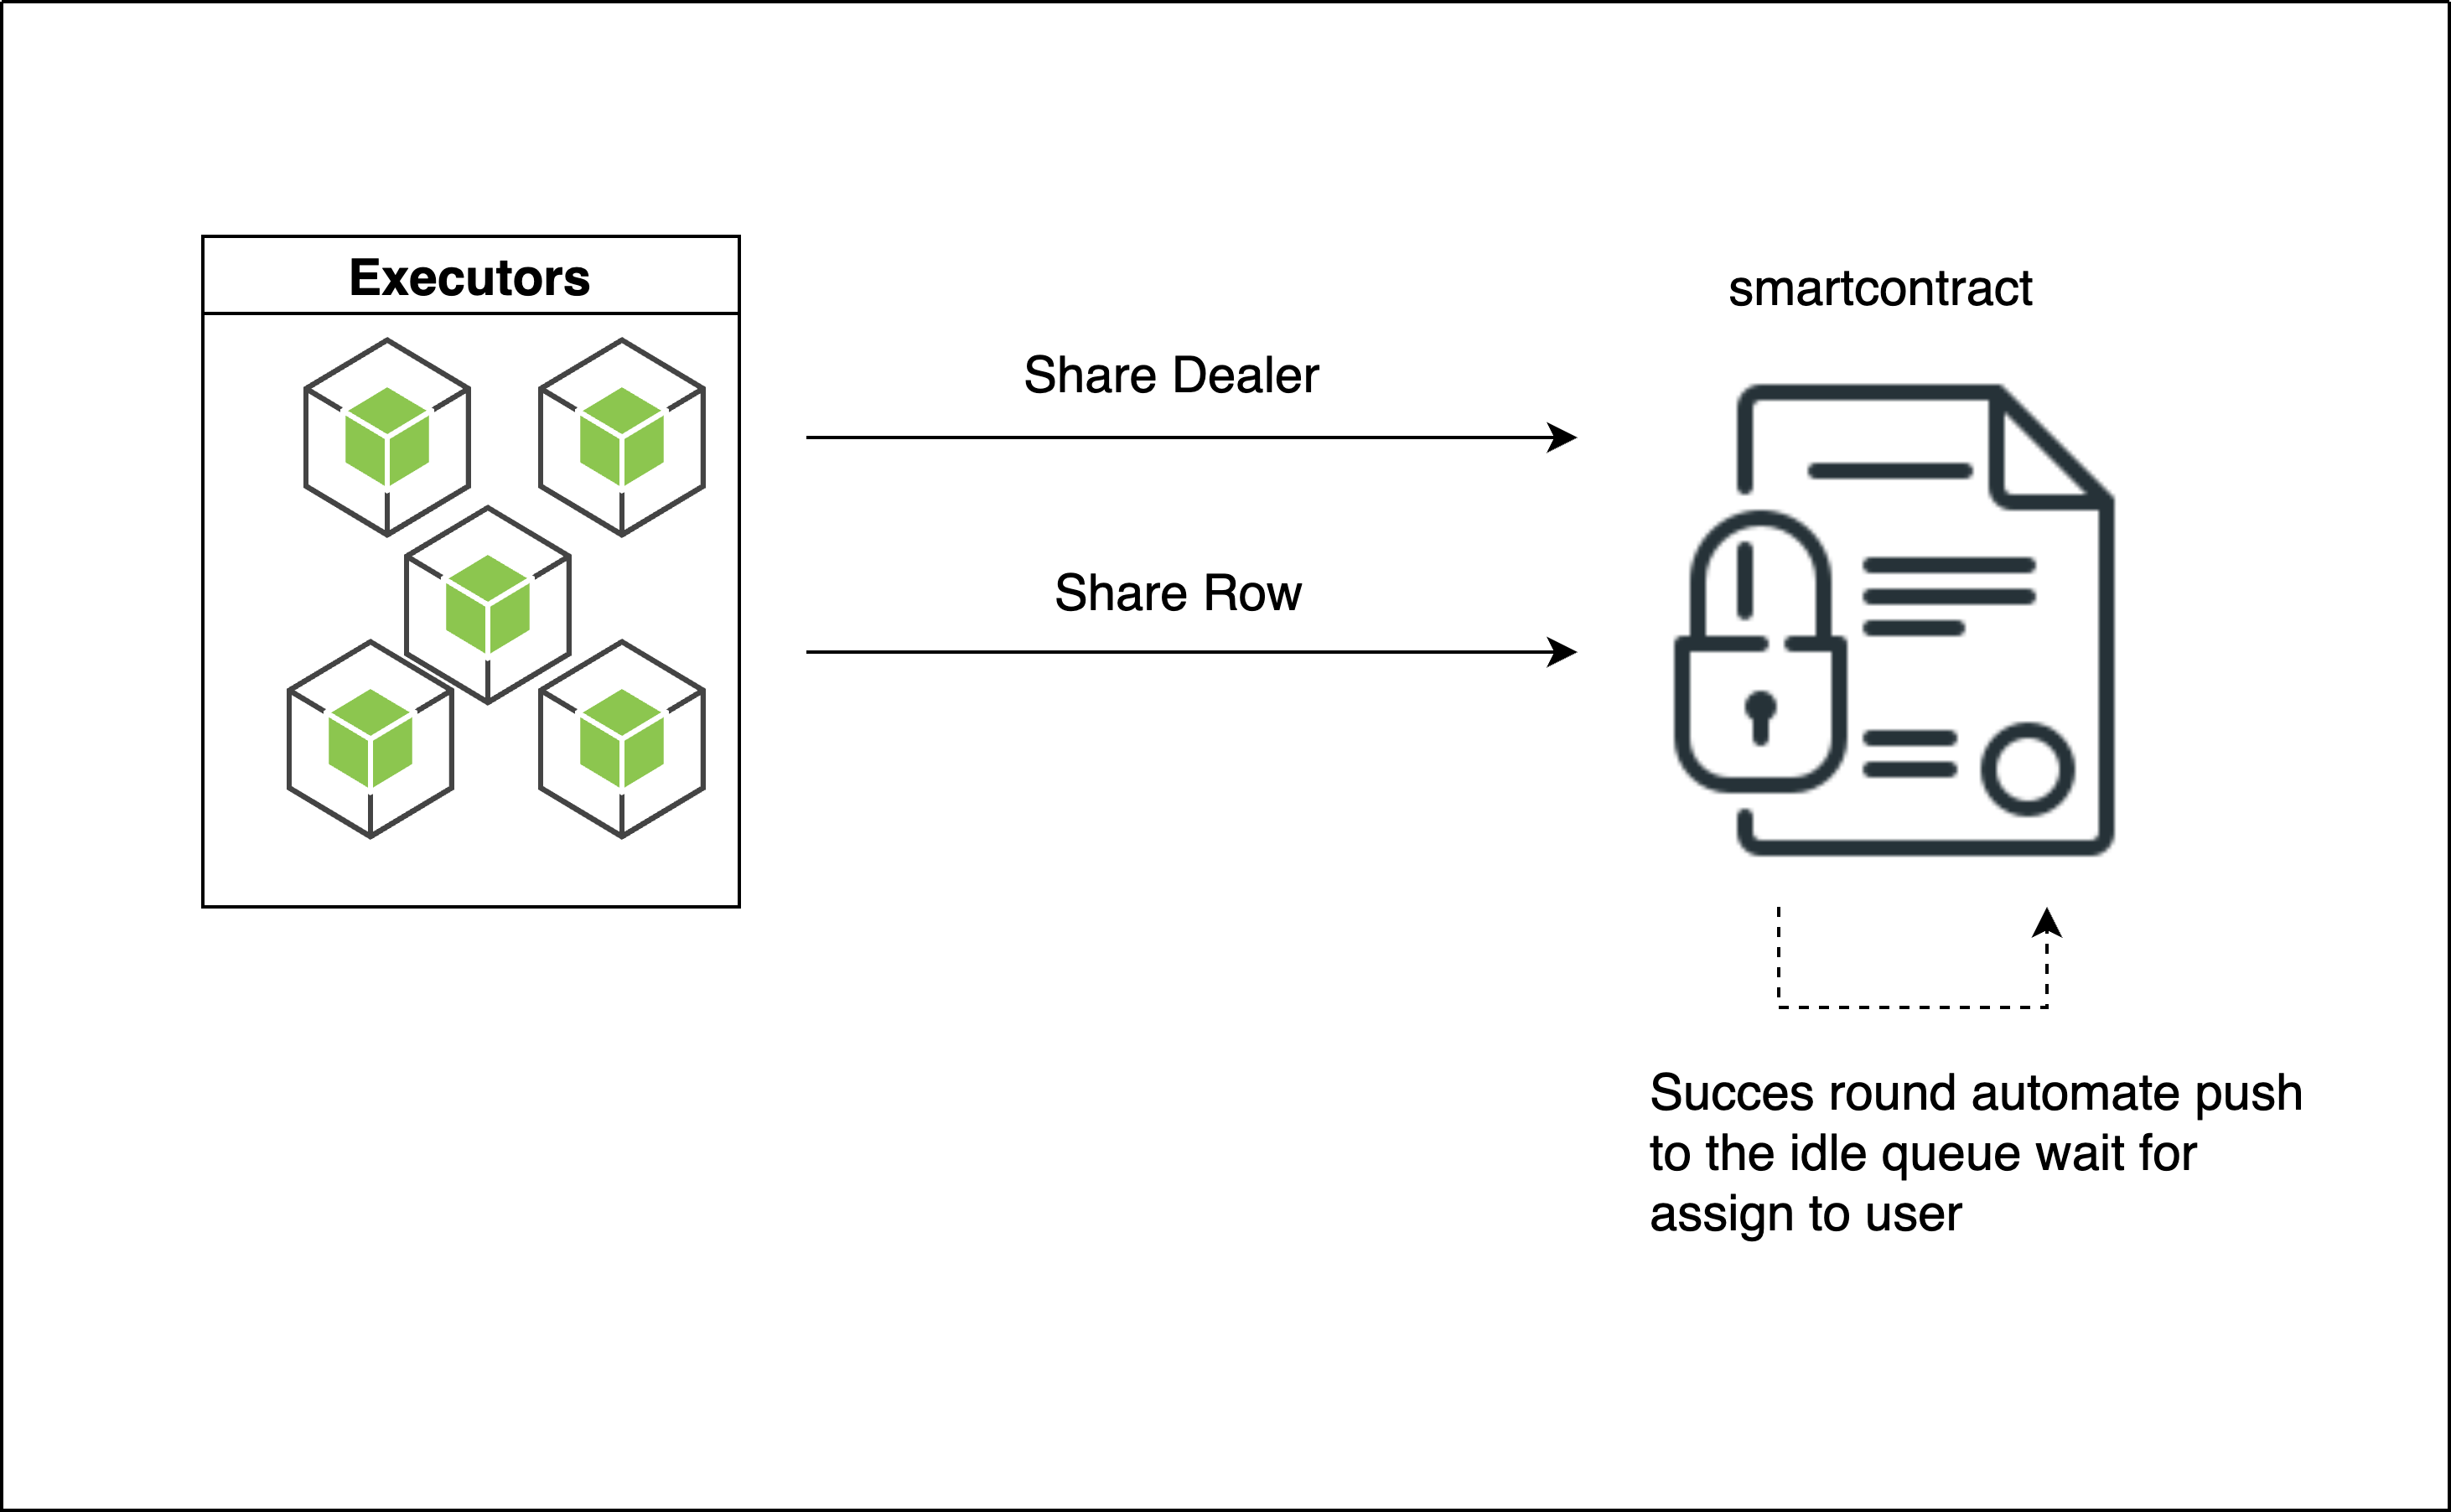
\includegraphics[scale=0.14]{Figure/executor-contribute.png}
 \caption{Asynchronous create encKey}
    \label{fig:create-encKey}
\end{figure}
The asynchronous creation of the encKey process is a crucial component of the architecture of the entire system, which is intended to maximize efficiency and resource utilization. By pre-generating a pool of idle encKeys, the system ensures that users can be assigned keys swiftly and seamlessly, without running the Distributed Key Generation (DKG) protocol each time. Executors, who are responsible for administering the encKey generation process, initiate the procedure. They continuously monitor the status of the current round and the number of inactive keys. When the system detects a need for new keys, such as when the present state is null or in the waitfordealer phase, and the number of idle keys falls below the expected threshold, the executors initiate the next round. During the initial phase of the round, known as the "sharing dealer" phase, the executors pool their individual confidential shares and share them with the designated sharing dealer. This phase ensures that each executor contributes without divulging sensitive information to the overall secret key. By collaborating, the executors distribute the secret shares in a manner that preserves the keys' security and integrity. Once the sharing dealer phase is successfully concluded, the protocol advances to the next phase, known as "waitforrows." In this phase, the executors use the shared secrets obtained in the preceding phase to generate their own public key shares. These public key shares are essential to the completion of the key generation process, as they assure the authenticity and validity of the user-assigned keys. The executors are well-prepared for the assignment of encKeys to users following the conclusion of the "waitforrows" phase. When a user requests their key, the system seamlessly maps the correct round to their designated key and provides it. This asynchronous approach to encKey creation improves the system's overall performance by decreasing the time and computational resources necessary for key assignment. The system accomplishes a seamless and secure workflow for encKey generation and assignment by incorporating the power of the DKG protocol and the efficiency of the asynchronous creation process. This method not only assures efficient resource utilization, but also improves the system's scalability and performance, allowing it to effectively handle a large number of user requests.


\end{document}
